\documentclass{beamer}

% german content
\usepackage[ngerman]{babel}

% bibliography
\usepackage[
  backend=biber,
  style=authoryear,
  citestyle=authoryear,
  autocite=footnote
]{biblatex}
\addbibresource{bibliography.bib}

% images
\usepackage{graphicx}
\graphicspath{ {./images/} }

\usepackage[normalem]{ulem}

\title{Peer-to-Peer Volltextsuche}
\subtitle{}
\author{
  Boris Caspary \\
  Emma Calewaert \\
  Jonathan Neidel \\
  Joscha Seelig \\
  Leon Enzenberger \\
  Ryan Torzynski \\
  Simon Breiter \\
  Stefan Sadewasser \\
}
\date{Juli 2021}
\institute{HTW Berlin, Angewandte Informatik, Projektstudium bei Herr Hoppe}
\logo{
\includegraphics[width=1cm]{logo}}

% theme + color theme
\usetheme{Szeged}
\usecolortheme{whale}
% see: https://deic-web.uab.cat/~iblanes/beamer_gallery/index.html
\setbeamerfont{caption}{size=\Tiny}

\begin{document}
\frame{\titlepage}

\section{Projektidee}
\begin{frame}
  \begin{center}
    {\Huge Projektidee}
  \end{center}
\end{frame}

\begin{frame}
  \frametitle{Bundestagsreden}
  \begin{itemize}
    \item Protokolle als Open Data verfügbar
    \item Großer Umfang an Daten
    \item XML-Dateien*
  \end{itemize}
\end{frame}

\begin{frame}
    \hspace*{-10.75mm}
    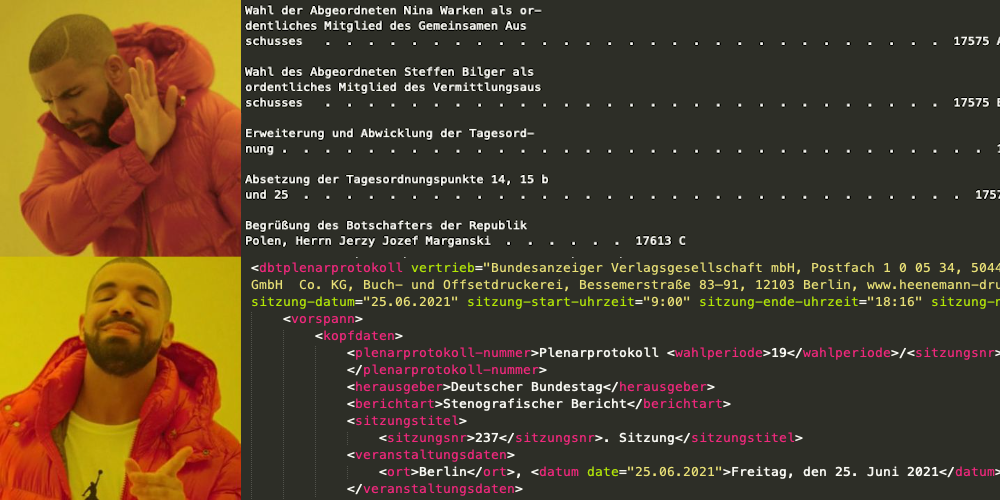
\includegraphics[width=\paperwidth]{drakememe}
\end{frame}

\begin{frame}[allowframebreaks]
  \frametitle{Basiskonzepte}
  Peer 2 Peer
  \begin{itemize}
    \item Rechnernetz
    \item Gleichtberechtigte Knoten
  \end{itemize}

  \break
  Volltextsuche
    \begin{itemize}
    \item Finden von Wörtern
    \item Handelt sich um Texte
    \item Zwei Phasen: Indexierung- und Anfragephase
  \end{itemize}
\end{frame}

\section{Arbeitsteilung}
\begin{frame}
  \begin{center}
    {\Huge Arbeitsteilung}
  \end{center}
\end{frame}

\begin{frame}[allowframebreaks]
  \frametitle{Arbeitspakete}

  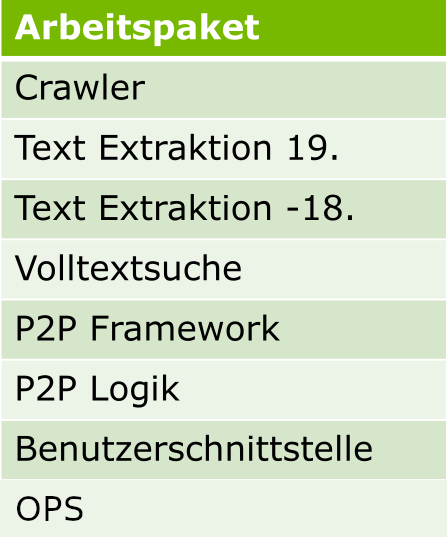
\includegraphics[width=5cm]{Arbeitspakete}
  \break
  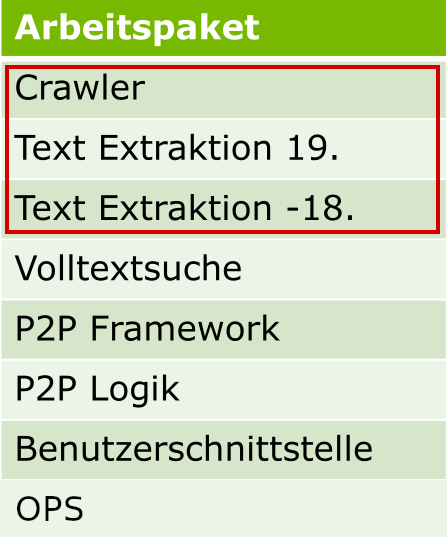
\includegraphics[width=5cm]{Arbeitspakete-Crawler}
  \break
  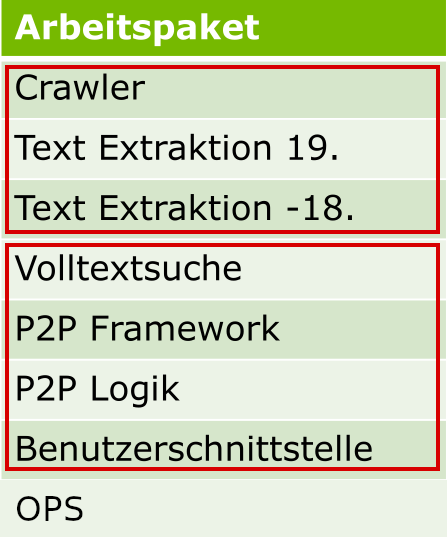
\includegraphics[width=5cm]{Arbeitspakete-Main}
  \break
  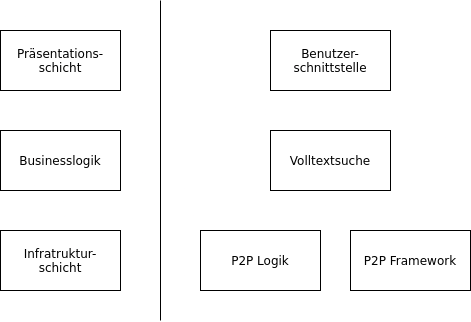
\includegraphics[width=8cm]{Schichten}
\end{frame}


\section{Peer-to-Peer}
\begin{frame}
  \frametitle{Peer-to-Peer}
  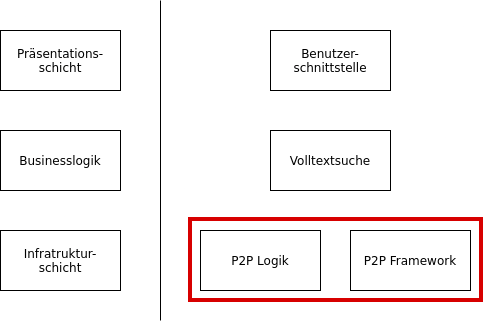
\includegraphics[width=8cm]{Schichten-p2p}
\end{frame}

\begin{frame}
  \frametitle{DHT}

  \begin{itemize}
    \item Distributed
    \item Hash Table
  \end{itemize}
\end{frame}

\begin{frame}
  \frametitle{Hash Table}

  \begin{itemize}
    \item key-value store
  \end{itemize}

  \medskip
  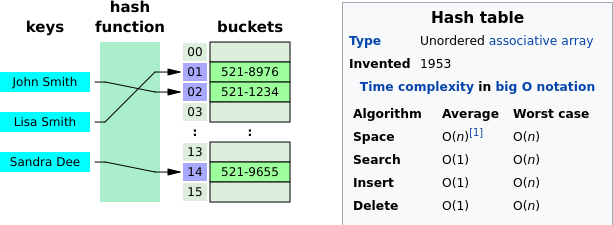
\includegraphics[width=8cm]{ht}
\end{frame}

\begin{frame}[allowframebreaks]
  \frametitle{Distributed HT}

  
\includegraphics[width=8cm]{dht1}

  \break

  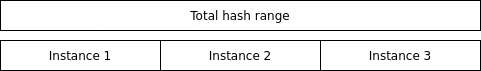
\includegraphics[width=8cm]{dht2}

  \break

  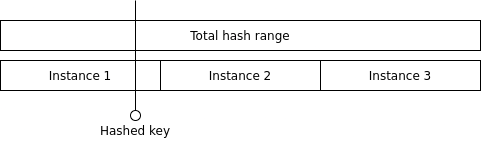
\includegraphics[width=8cm]{dht3}
\end{frame}

\begin{frame}
  \frametitle{Schichten}

  \begin{center}
    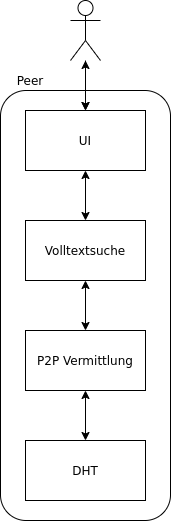
\includegraphics[height=6cm]{Schichten-alt}
  \end{center}
\end{frame}

\begin{frame}
  \frametitle{Verteilung des Systems}

  Design Entscheidung:

  Wie soll die Funktionalität des Systems verteilt werden?
\end{frame}

\begin{frame}[allowframebreaks]
  \frametitle{1. Zentralisierung}

  \begin{center}
    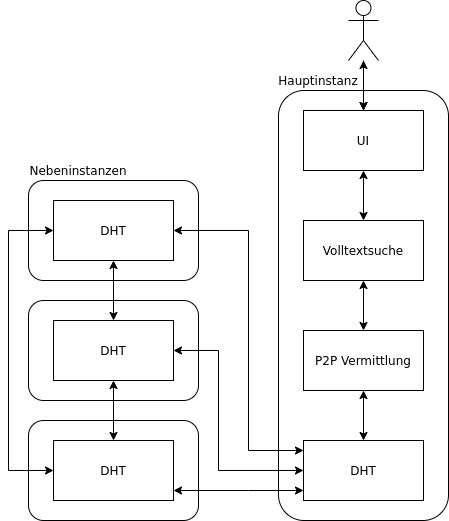
\includegraphics[height=6cm]{Hauptinstanz}
  \end{center}

  \break
  Pro:
  \begin{itemize}
    \item zentrale Anlaufstelle (Nutzerfreundlich)
  \end{itemize}

  Con:
  \begin{itemize}
    \item zentrale Anlaufstelle (single point of failure)
    \item Load nicht verteilt
  \end{itemize}
\end{frame}

\begin{frame}[allowframebreaks]
  \frametitle{2. Pur}

  \begin{center}
    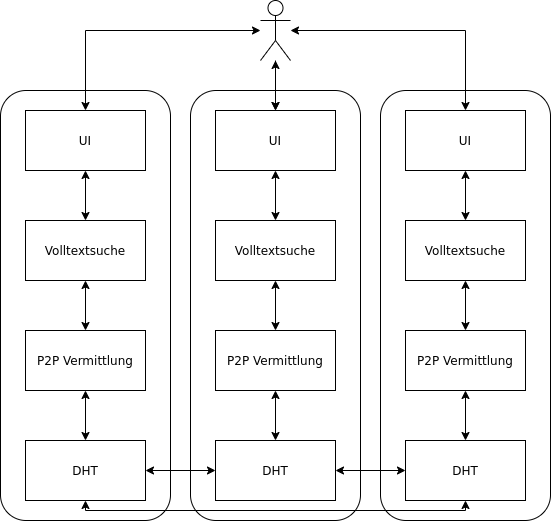
\includegraphics[height=6cm]{Gleichberechtigt}
  \end{center}

  \break
  Pro:
  \begin{itemize}
    \item Load verteilt
    \item mehrere Anlaufstellen (kein single point of failure)
  \end{itemize}

  Con:
  \begin{itemize}
    \item mehrere Anlaufstellen (verwirrte Nutzer $\rightarrow$ Loadbalancer)
    \item Administrationsaufwand ($\rightarrow$ OPS)
  \end{itemize}
\end{frame}

\section{Volltextsuche}
\begin{frame}
  \frametitle{Volltextsuche}

  \begin{center}
    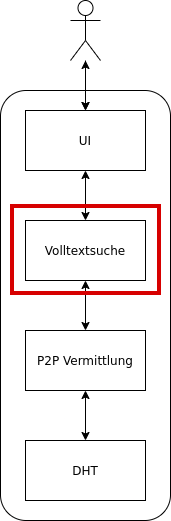
\includegraphics[height=6cm]{Schichten-alt-volltext}
  \end{center}
\end{frame}

\begin{frame}
  \frametitle{Volltextsuche}

  Modi:
  \begin{enumerate}[I]
    \item Vorbereiten und Einfügen von Daten
    \item Abrufen von Daten
  \end{enumerate}
\end{frame}

\begin{frame}[allowframebreaks]
  \frametitle{I. Vorbereiten von Daten}

  Beispiel:

  Klaus-Rüdiger steht vor dem Hause der CDU.

  \break

  \textbf{Tokenisierung:}

  Segmentierung in einzelne Wörter

  \bigskip
  'Klaus-Rüdiger' 'steht' 'vor' 'dem' 'Hause' 'der' 'CDU'

  \break

  \textbf{Füllwörter entfernen:}

  \begin{itemize}
    \item Pronomen (ich, ihre, ..)
    \item Konjunktionen (und, aber, ..)
    \item Präposition (auf, bis, ..)
    \item Artikel (der, die, ..)
  \end{itemize}

  \bigskip

  'Klaus-Rüdiger' 'steht' \sout{'vor'} \sout{'dem'} 'Hause' \sout{'der'} 'CDU'

  \break

  \textbf{Stemming:}

  \bigskip

  Zurückführung auf den Wortstamm:

  \medskip

  Häuser $\rightarrow$ Haus

  \bigskip
  'Klaus-Rüdiger' \textbf{'steht' $\rightarrow$ 'stehen'} \textbf{'Hause' $\rightarrow$ 'Haus'} 'CDU'

  \break

  \textbf{Normalisierung:}

  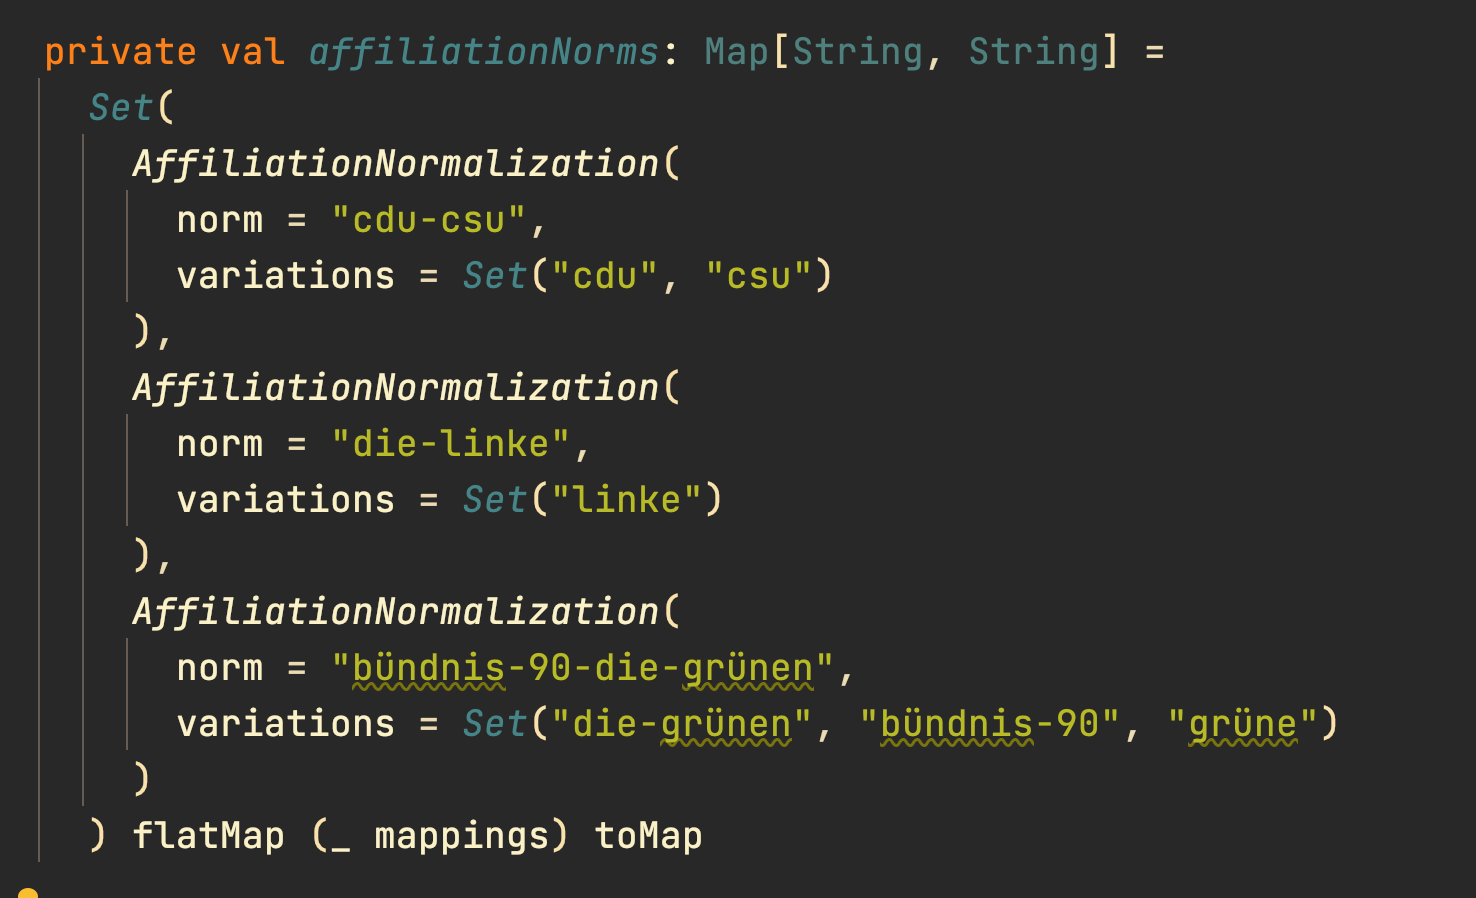
\includegraphics[width=8cm]{normalisierung}

  \bigskip
  'Klaus-Rüdiger' 'stehen' 'Haus' \textbf{'CDU' $\rightarrow$ 'cdu-csu'}
\end{frame}

\begin{frame}
  \frametitle{I. Einfügen von Daten}

  \begin{itemize}
    \item in invertierten Index
    \item verteilt durch DHT
  \end{itemize}
\end{frame}

\begin{frame}
  \frametitle{Invertierter Index}

  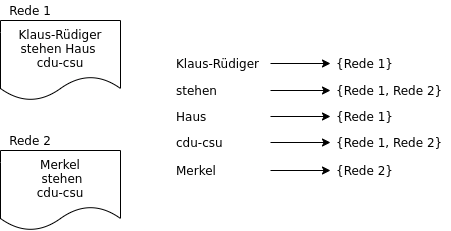
\includegraphics[width=8cm]{inverted-index}
\end{frame}

\begin{frame}[allowframebreaks]
  \frametitle{I. Verteilung der Daten}

  Design Entscheidung:

  Wie sollen die Daten verteilt werden?

  \break

  \textbf{1. Nach Partei}

  Ein Sever zuständig für eine Partei

  Pro:
  \begin{itemize}
    \item Schnell beim Einfügen
    \item Schnell beim Abrufen wenn nach Partei gefiltert
  \end{itemize}
  Con:
  \begin{itemize}
    \item Sonst langsam
    \item Load Imbalance
  \end{itemize}

  \break

  \textbf{2. Nach Keyword}

  Gleichmäßige Verteilung

  Pro:
  \begin{itemize}
    \item Schnell beim Abrufen von Keywords
    \item Load Balance
  \end{itemize}

  Con:
  \begin{itemize}
    \item Langsam bei Partei Filterung ($\rightarrow$ Restriktion)
    \item Langsam beim Einfügen
  \end{itemize}
\end{frame}

\begin{frame}
  \frametitle{II. Abrufen von Daten}

  \begin{itemize}
    \item Abholen der Daten aus invertiertem Index
    \item Bewertung der Relevanz (sortieren)
  \end{itemize}
\end{frame}

\section{Demo}
\begin{frame}
  \frametitle{UI Demo}

  \begin{center}
    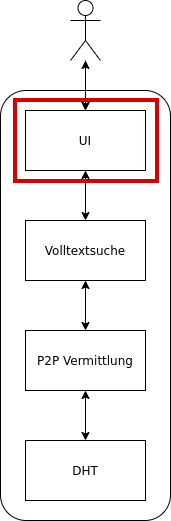
\includegraphics[height=6cm]{Schichten-alt-ui}
  \end{center}
\end{frame}

\end{document}
